\documentclass[11pt,a4paper]{article}
\usepackage{amsmath}
\usepackage{amssymb}
\usepackage{graphicx}
\usepackage{color}
\usepackage{fancyhdr}
\usepackage[margin=3.5cm]{geometry}
\usepackage{framed}
\usepackage{enumerate}
\usepackage{textcomp}
\usepackage{fancyvrb}

\usepackage[colorlinks=true,urlcolor=blue,citecolor=black,linkcolor=black]{hyperref}
\def\ket#1{\left|#1\right\rangle}
\def\bra#1{\left\langle#1\right|}
\def\braket#1{\left\langle#1\right\rangle}

\newcommand{\sepline}{%
  \hspace{0.3\textwidth}\rule{0.5\linewidth}{.7pt}\hspace{0.3\textwidth}%
}

\fancyhf{}
\lhead{NTU/SPMS/PH2198--PH2199 Lab}
\rhead{Writing a Good Lab Report}
\lfoot{\tiny\textcopyright \;2018 Nanyang Technological University.  Released under \href{http://creativecommons.org/licenses/by-sa/4.0/}{CC BY-SA 4.0}.}
\rfoot{\thepage}
\pagestyle{fancy}

\definecolor{dgreen}{RGB}{70,128,13}

\begin{document}

\begin{center}
\textbf{Division of Physics\;\,\&\;Applied Physics}

\textbf{PH2198/2199---Physics Laboratory IIA/IIB}

\vskip 0.05in

\underline{\Huge Writing a Good Lab Report}
\end{center}

\section{What is---and isn't---a proper lab report}

The lab reports that you will prepare in this course are shorter and
simpler versions of the reports that working scientists use to
communicate their findings.  Such reports are expected to be accurate,
complete, concise, and readable.

\begin{itemize}
\item \textit{Accurate}---The contents must be unambiguous and
  correct.  ``Correct'', in this context, means that the contents
  match what happened during the experiment; it does not mean
  ``getting the right answer''.  It is OK to have results that are
  uncertain or that do not match expectations, provided these
  uncertainties and deviations are pointed out and/or explained.

\item \textit{Complete}---The report must include all information a
  reader would reasonably want.  For example, if you use a symbol in
  an equation, figure, or text, that symbol should be defined (in a
  caption or in the text).  If you show a plot of experimental
  results, the text should describe how the data were obtained, and
  what conclusions the reader should draw from it.

\item \textit{Concise}---Do not clutter the report with useless
  information.  Assume that the reader is scientifically literate (at
  the level of a fellow physics undergraduate).  For instance, you
  need not explain classical mechanics before talking about forces.
  Omit details that most readers would consider trivial (e.g., the
  fact that the voltage on a power supply increases when turning a
  dial clockwise).

\item \textit{Readable}---The text in the lab report must form a
  coherent, readable narrative.  The main text should form proper
  paragraphs.  Do not write your report in Q\&A (question-and-answer)
  form, and do not organize your report as a mere collection of
  bullet-point lists.  Your descriptions of experimental procedures
  shouldn't be a list of steps lifted from the lab manual; that
  information should be converted into proper paragraphs, and
  interwoven with explanations about the intention of the procedures,
  what happened during the experiment, etc.
\end{itemize}

\noindent
The best way to internalize these criteria is to always bear in mind
the goal of a lab report, which is to communicate a set of scientific
findings to interested parties.  Readers will be happy if the
information is presented clearly and accurately, and contains all the
details that they need to understand the results.  They will be
annoyed if you write about irrelevancies, or format the report in an
inscrutable way.

\section{Sections of the report}

Your lab report should be divided into distinct sections.  There is no
standard set or sequence of sections.  Here is a typical and
acceptable outline:

\begin{enumerate}
\item \textit{Introduction}---A description of the goals of the
  experiment.  Do not lift the text from the lab manual; use your own
  words.  The introduction need not be long; in many cases, one or two
  paragraphs is enough.

\item \textit{Methods}---Descriptions of the experimental set-up and
  procedures.  When writing about the set-up, do not follow the lab
  manual in listing out individual pieces of equipment and assembly
  instructions; that's not relevant information in a lab report!
  Instead, describe the apparatus as a whole (preferably with a
  diagram), and explain how it works.

  Likewise, when describing the experimental procedure, do not simply
  lift instructions from the lab manual.  Your description should take
  the form of a narrative, and include information not present in the
  manual, such as descriptions of what happened during intermediate
  steps of the experiment.

\item \textit{Results}---This section should contain \textit{both}
  complete paragraphs of text \textit{and} figures/tables.  The text
  paragraphs should be written in such a way that it is possible to
  understand what's going on by just reading through them, without
  looking at the figures.  Every figure/table must be referenced and
  discussed somewhere in the text (e.g., ``\textit{The dependence of
    the sample temperature on applied voltage is plotted in Fig.~3.
    From the data, we observe an approximately linear relationship.  A
    linear least squares fit shows that...}'').

  The report should contain all necessary details about how the data
  were analyzed, including error analysis (i.e., derivations for the
  uncertainty estimates).  If an analysis is too long, relegate it to
  an appendix.

\item \textit{Conclusions}---Summary of what was learnt from the
  experiment.  If the results seem unexpected or unreliable, discuss
  them and give possible explanations.  This section need not be long;
  one or two paragraphs is OK.

\item \textit{Appendix A, Appendix B, etc.}---You can use appendices
  for detailed derivations, tables of raw data, etc., to avoid
  cluttering up the main text.

\item \textit{References}---If you referred to any other works in the
  text of the report, list them here.  References should be numbered,
  and appear in the same order they are mentioned in the text.  The
  text should cite references by number.
\end{enumerate}

\noindent
You don't need to stick religiously to this outline.  For example, in
some cases, instead of \textit{Methods} and \textit{Results} sections,
it might be better to divide the experiment into several conceptually
distinct parts, and describe the methods and results for each part
within a single section.

Some lab manuals provide an explicit list of issues/questions to be
addressed in your report.  \underline{Do not create a
  Question-and-Answer section for this.}  Instead, deal with these
issues at appropriate places in your report; it is up to you to decide
where.  For example, if there is a question about safety hazards and
how to mitigate them, it might be appropriate to have one or two
paragraphs discussing this in the \textit{Methods} section, during
your description of experimental procedures.

\section{Figures}

You are free to choose the software for preparing the figures in your
lab report.  The software must be able to produce plots of
professional scientific quality, including horizontal and vertical
error bars, text labels, multiple curve and data point types, and
logarithmically-scaled axes.  We specifically recommend Python's
\href{https://matplotlib.org/}{Matplotlib} module,
\href{https://www.gnu.org/software/octave/}{GNU Octave},
\href{https://www.mathworks.com/products/matlab.html}{Matlab}, or
\href{https://www.originlab.com/}{Origin} (the first two are free).

Here are some issues to watch out for when making plots:

\begin{itemize}
\item All data points must have error bars---preferably both vertical
  and horizontal error bars---unless there's a good reason otherwise.

\item Axes must be clearly titled, including units.  If space permits,
  axis titles should have descriptive text, not just symbols; e.g.,
  ``Applied force $F$ (mN)'' is better than ``$F$ (mN)''.

\item If a graph has multiple sets of curves/data points, they must be
  distinguishable (e.g., solid versus dashed curves, or circular
  versus triangular data points).  The different sets should be
  labeled in the figure and/or described in the caption.

\item The figure must have a caption describing its contents.  Never
  worry about putting ``too much'' in the captions; in particular, it
  is OK to have overlap between the contents of the caption and the
  main text.

\item
  All text in the figure (including the legends, axis labels, and axis
  titles) must be big enough to read.  As a rule of thumb, figure text
  should be 60--100\% the size of the regular text in the manuscript,
  and no smaller.  If your plotting program produces text that's too
  small by default, adjust it yourself.
\end{itemize}
\noindent
An example of a good figure is shown in Fig.~\ref{pendulum-figure-1}.
Note the error bars, the axis titles and labels (which are in legible
sizes, with units), and the description of the best-fit line in the
caption.  Some examples of bad figures are given in
Appendix~\ref{sec:bad-examples}.

\begin{figure}[h]
  \centering
  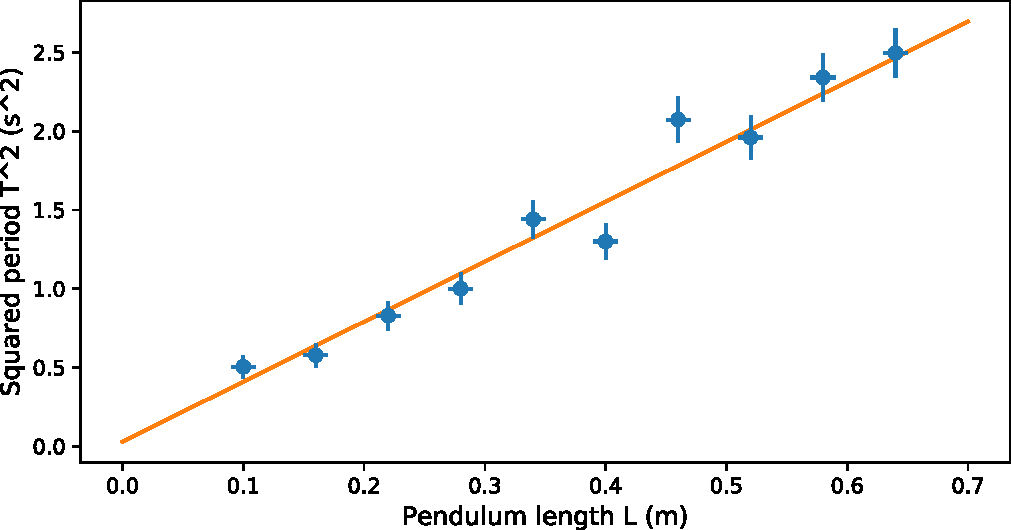
\includegraphics[width=0.8\textwidth]{pendulum-figure-1.pdf} \\
  \caption{\small [Example of a good figure.]  Plot of squared
    pendulum period $T^2$ versus pendulum arm length $L$.  The solid
    orange line shows the linear least-squares fit, which yields an
    estimated gravitational constant of $g \approx 10.4 \pm
    0.7\,\textrm{ms}^{-2}$.}
  \label{pendulum-figure-1}
\end{figure}

\section{Miscellaneous Issues}

\begin{itemize}

\item \textit{Figures from the lab manual}---You may excerpt figures
  from the lab manual, where appropriate.  However, the figure caption
  must note that the figure is from the lab manual, with an
  appropriate citation/reference.

\item \textit{Page and figure/table/equation/section numbering}---All
  pages should be numbered, and so should figures, tables, equations,
  and sections.  Refer to these numbers whenever possible; e.g.,
  ``\textit{as described in Section 2...}'' instead of ``\textit{as
    described above...}''

\item \textit{Curve fits must make sense}---When fitting data, you
  should be able to justify the type of curve you are using (e.g.,
  based on theory).  It is a mistake to simply fit to a high-order
  polynomial, like in Fig.~\ref{bad-curve-fit}, without any idea
  whether the ``actual'' curve ought to have such a form.  Such a fit
  might look nice, but it supplies no actual information!
  
  \begin{figure}[h]
  \centering
  \fbox{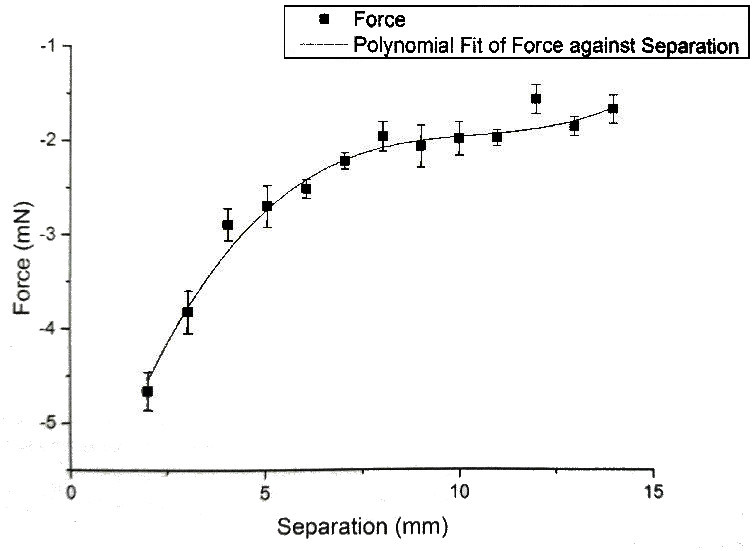
\includegraphics[width=0.5\textwidth]{bad-curve-fit.jpg}} \\
  \caption{\small An example of a curve fit that makes no sense.}
  \label{bad-curve-fit}
\end{figure}

  
\item \textit{Raw data}---Include your raw experimental data in table
  form, with proper captions and column headings (including units and
  uncertainties).  If the table is quite large, put it in an appendix.
  If there is truly too much raw data to put into the report, you may
  omit it, but in that case you must bring the raw data (in hardcopy
  or electronic form) to the viva.  You must be able to provide the
  raw data on request anytime during the semester, so do not dispose
  of it until after the semester, when you have received a grade for
  the course.

\item \textit{Length}---Lab reports in this course typically need not
  exceed 7 pages.  Use $\approx 11 $ point fonts, with normal
  (\textit{not} double) line spacing.
\end{itemize}


\pagebreak

\begin{center}
  {\LARGE \textbf{Appendix}}
\end{center}

\appendix
\section{Good and Bad Examples}
\label{sec:bad-examples}

Here are some examples showing good and bad practices in lab reports.

\begin{figure}[h]
  \centering
  \fbox{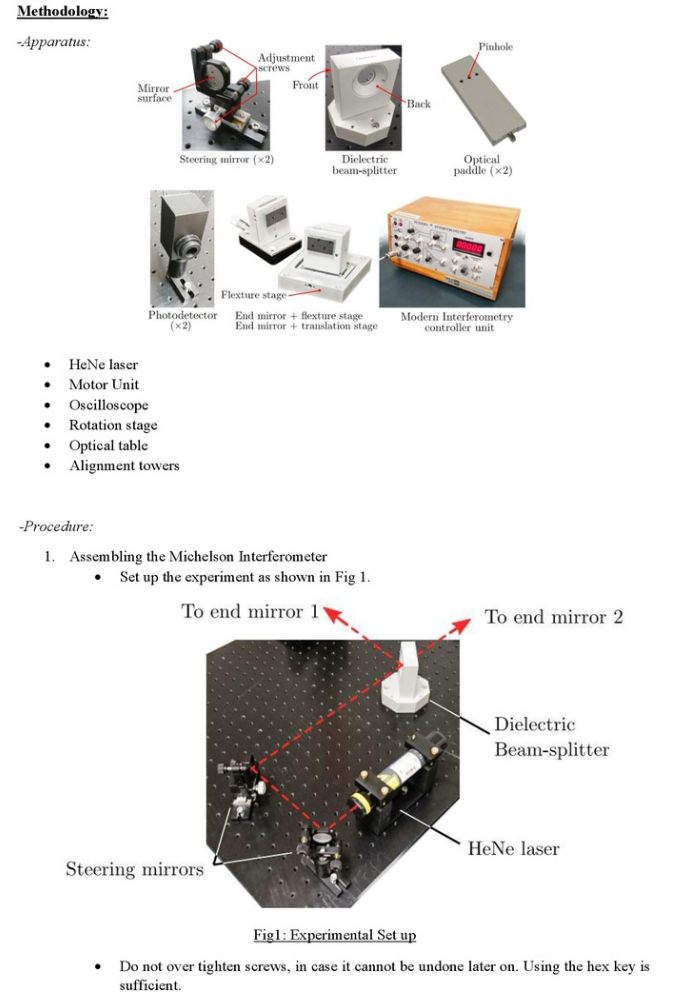
\includegraphics[width=0.73\textwidth]{bad-example-1.png}} \\
  \caption{\small \textbf{Bad example}.  Here, the ``Apparatus'' and
    ``Procedure'' sections are essentially lifted from the lab manual,
    which is unacceptable.  The pictures are from the lab manual,
    which ought to be cited.  The equipment list and assembly
    instructions are irrelevant; only the assembled apparatus ought to
    be described.  The text should consist of complete paragraphs, not
    bullet-point lists.  }
\end{figure}

\begin{figure}[h]
  \centering
  \fbox{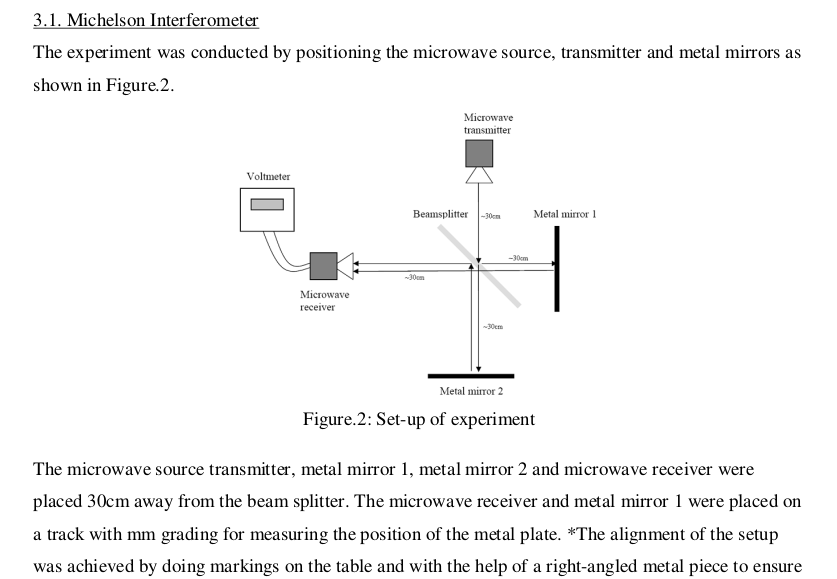
\includegraphics[width=0.85\textwidth]{good-writeup.png}} \\
  \caption{\small \textbf{Good example}.  The experimental setup is
    shown in a schematic figure, and is then explained clearly and
    concisely in the main text.}
\end{figure}


\begin{figure}
  \centering
  \fbox{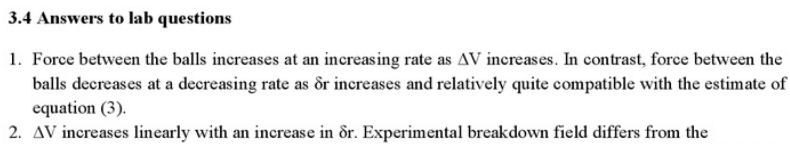
\includegraphics[width=0.85\textwidth]{bad-example-4.png}} \\
  \caption{\small \textbf{Bad example} A separate section has been set
    aside for answering the lab manual's question list.  Please
    instead address the questions at relevant points in the report.}
\end{figure}

\begin{figure}[h]
  \centering
  \fbox{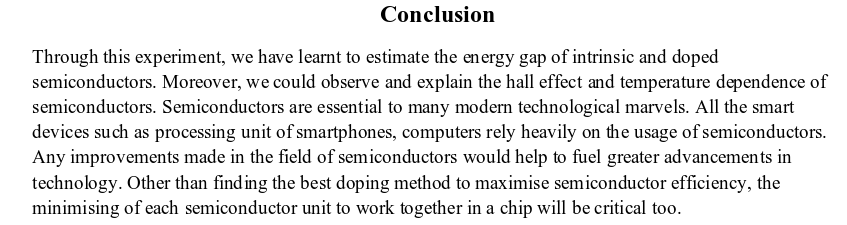
\includegraphics[width=0.85\textwidth]{bad-conclusion.png}} \\
  \caption{\small \textbf{Bad example}.  The conclusion is too
    qualitative, and too much of it is spent discussing issues outside
    the scope of the experiment.}
\end{figure}

\begin{figure}[h]
  \centering
  \fbox{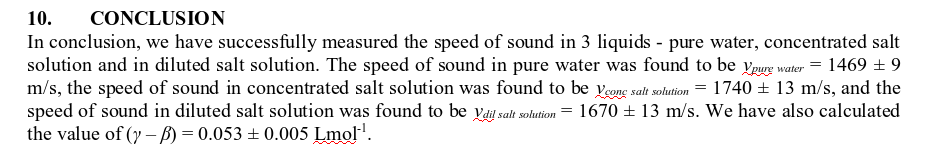
\includegraphics[width=0.85\textwidth]{good-conclusion.png}}
  \\
  \caption{\small \textbf{Good example}.  The experimental results are
    summarized clearly and precisely.}
\end{figure}

\begin{figure}
  \centering
  \fbox{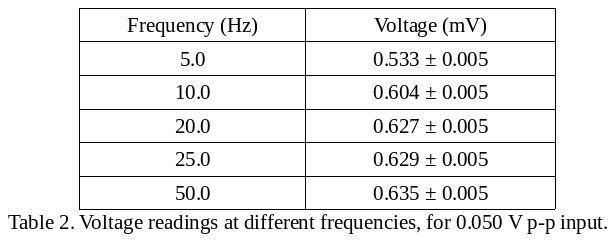
\includegraphics[width=0.6\textwidth]{good-table.png}} \\
  \caption{\small \textbf{Good example}.  This data table has clear
    column headings with both descriptive text and units. Measured
    quantities include error estimates (reported to one significant
    figure), and in each reported value the number of digits matches
    the error. }
\end{figure}


\begin{figure}
  \centering
  \fbox{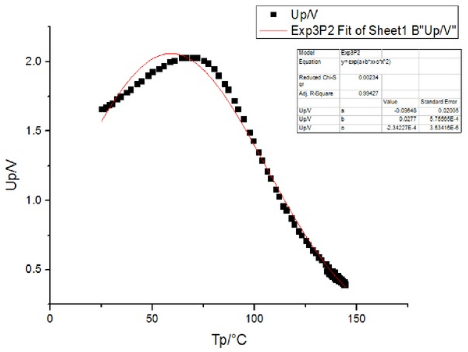
\includegraphics[width=0.6\textwidth]{bad-example-2.png}} \\
  \caption{\small \textbf{Bad example}.  The text in the lower box is
    too small to read.  Any text appearing in a figure is assumed to
    be relevant, and should thus be legible; if the text is
    irrelevant, omit it.  Also, the data points should have error
    bars.}
\end{figure}

\begin{figure}
  \centering
  \fbox{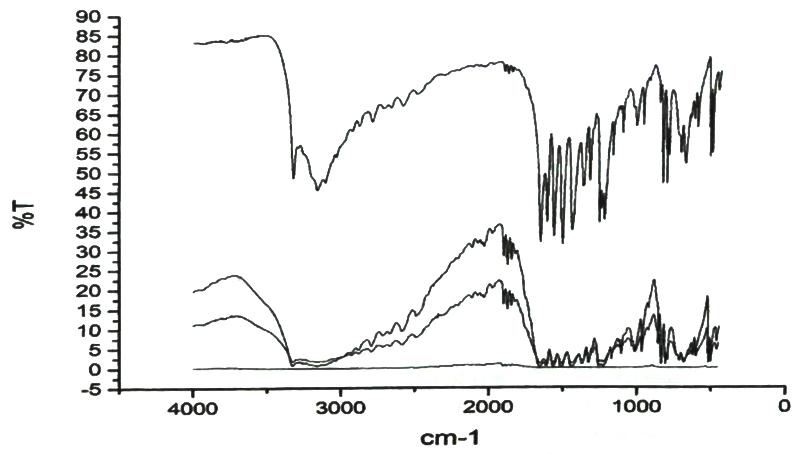
\includegraphics[width=0.6\textwidth]{bad-example-3.png}} \\
  \caption{\small \textbf{Bad example}.  Here, three different data
    sets are plotted with indistinguishable lines; instead, different
    line types should be used, and clearly labelled.  Also, the
    horizontal axis should have a proper title (text description and
    symbol, not just a unit).  The vertical axis should have a text
    description, not just a symbol.  }
\end{figure}



\end{document}
